\appendix
\sloppy

This appendix preserves protocol and diagnostic details omitted from the eight-page main submission. All quantities derive from the same frozen experimental records underlying the main paper.

\section*{Endpoint status and amendments}

The table below separates outcomes fixed before provider execution from later analytical qualifications. The qualifications preserve the frozen runs and report rather than replace the original records.

\begin{center}
\resizebox{\columnwidth}{!}{%
\scriptsize
\begin{tabular}{>{\raggedright\arraybackslash}p{0.22\columnwidth}>{\raggedright\arraybackslash}p{0.29\columnwidth}>{\raggedright\arraybackslash}p{0.39\columnwidth}}
\toprule
\shortstack{\textbf{Component}} & \shortstack{\textbf{Frozen}\\\textbf{endpoint}} & \shortstack{\textbf{Final status or}\\\textbf{qualification}} \\
\midrule
Canary audit & Post-input exact or five-token partial exposure in the three-arm 120-instance replication & 0/120 in evolve and reset, and 0/120 false positives in no-canary; one-sided 95\% upper bound 2.5\%, reported as failed to detect for the audited setting. \\
Length ablation & Paired exactness and recorded-score differences in each frozen cohort & Cohort results are primary; the 42-pair synthesis was added after cohort inspection and is labeled secondary and outcome-aware. \\
Fixed-pool headroom & Oracle over the recorded candidate surface & Final answers were retained in the support set by an explicit amendment; the pooled cross-cohort summary remains exploratory. \\
Nested trajectory pool & Support and oracle differences for $C_1\subset C_5$ & Nested sign tests were withdrawn because decreases are impossible by construction; task-bootstrap intervals and one-sided bounds were retained. The matched decomposition is slot-matched, not token-matched. \\
Repair gate & Restart versus repair after shared-anchor failure & The stop rule was reached with three informative failures, so no main cohort was run; the result is a stopped diagnostic. \\
Task-level response collapse & Same-task public-only control on the two exhausted tasks & The control was frozen before those calls; the two tasks remain selected mechanism cases, not a population sample. \\
Selector calculation & Closed-form exponential-mechanism probabilities on cached candidates & This is an illustrative narrow-adjacency calculation, not an empirical end-to-end DP experiment. \\
\bottomrule
\end{tabular}%
}
\end{center}

\section{Audit procedure and stop rules}
\label{app:procedure}

The audit is an ordered checklist. Each step has an estimand, a stop rule fixed before the corresponding run, and an escalation rule; the thresholds below are the ones used in this study, not universal defaults.

\begin{enumerate}
  \setlength{\itemsep}{1pt}
  \item \textbf{Exposure.} Estimand: post-input exact or five-token partial canary recovery, evolve versus depth-matched reset. Signal rule (protocol 199): evolve exposure at least 10\%, a positive paired difference, and exact McNemar $p<0.05$ over 120 complete triads. If not met, report a bounded non-detection and do not calibrate privacy for that channel.
  \item \textbf{Score consequence.} Estimand: paired difference in executable or reference exactness when the score term is removed, with a manipulation check on the score itself. The frozen rules check the score scale first and then a utility-improvement criterion; we report a utility interval that contains zero as inconclusive, never as score invalidity. The frozen precise-null rule for the pooled synthesis requires an interval containing zero with upper endpoint below 0.15.
  \item \textbf{Realized support.} Estimand: the hindsight oracle gap $H_i$ over the recorded pool. Rule (protocol 077): fewer than 4/20 recoverable failures stops selector or retention development on that pool.
  \item \textbf{Support expansion.} Only if step 3 stops: enlarge the pool prospectively and re-measure $H_i$ and cost before any private-selection experiment.
\end{enumerate}

Minimum detectable effects follow from the sample sizes: with 120 complete triads, the planning simulation for step 1 gives 94.8\% power for 15\% versus 2\% discordance; with 20 pairs, step 2 needs at least five pure discordances for one-sided exact $p<0.05$ (Appendix~\ref{app:null}). Cost is reported as provider-recorded tokens at every step.

\section{Metric definitions}
\label{app:metrics}

\begin{center}
\resizebox{\columnwidth}{!}{%
\scriptsize
\begin{tabular}{>{\raggedright\arraybackslash}p{0.20\columnwidth}>{\raggedright\arraybackslash}p{0.37\columnwidth}>{\raggedright\arraybackslash}p{0.14\columnwidth}>{\raggedright\arraybackslash}p{0.21\columnwidth}}
\toprule
\textbf{Metric} & \textbf{Definition} & \textbf{Needs reference} & \textbf{Used for} \\
\midrule
Executable validity & Parser-accepted canonical plan that the reference-free executor runs from the initial inventory to the target & No & Headroom, oracles, retention, selector \\
Reference exactness & Canonical final answer equals the reference action list or \texttt{IMPOSSIBLE} label & Yes (offline) & Length-term removal, Table~\ref{tab:audit} \\
Canonical exact & Plan identical to the canonical reference sequence & Yes (offline) & Planner (secondary) \\
Replay validity & Independent environment replay reaches the target & No & Planner, cross-checks \\
\bottomrule
\end{tabular}%
}
\end{center}

On the 65 eligible final answers of Table~\ref{tab:headroom}, executable validity and reference exactness agree in every run. A separate replay of all 48 non-degenerate DeepSeek finals through the public PlanCraft environment reaches the target in exactly the 26 reference-exact rows. Neither check tests parser false negatives on unparseable text.

\section{Threat model and trust boundary}
\label{app:threat}

The two privacy-relevant components answer different questions and use different boundaries.

\begin{center}
\resizebox{\columnwidth}{!}{%
\scriptsize
\begin{tabular}{>{\raggedright\arraybackslash}p{0.20\columnwidth}>{\raggedright\arraybackslash}p{0.36\columnwidth}>{\raggedright\arraybackslash}p{0.36\columnwidth}}
\toprule
& \textbf{Canary audit} & \textbf{Selector calculation} \\
\midrule
Protected unit & A synthetic random canary injected only in the round-one query & One candidate's clipped validity bit (candidate-score replacement adjacency) \\
Observer & Anyone who can read persistent state after the input round: memory, feedback, stored outputs, scores, and slow-update logs & Only the selected index or output \\
Released & Full state snapshots after the input round & The selected index or output \\
Trusted & Runtime code, provider, and extractor & Candidate texts, prompts, memories, messages, control flow, and the executor \\
Out of scope & Adaptive extraction, provider-side logs, structural edits, task-relevant secrets & End-to-end DP of the transcript or of the evolving state \\
\bottomrule
\end{tabular}%
}
\end{center}

A detected canary would show a persistence channel; a non-detection is a bounded failure to detect under this observer, not a guarantee against a stronger one.

\section{Score sources and per-arm consequences}
\label{app:scoreconsequence}

In the 60 initial canary-study runs (15 agent-round scores each), 705 of 900 recorded contribution scores are fast-round heuristic scores and 195 come from slow-update judging. Of the 165 observations scoring at least 0.8, 24 belong to the five successful runs, compared with 75 of 900 observations overall; these observations are clustered within runs. The run-level AUC of the maximum contribution score is 0.755, and the conditional interval in Appendix~\ref{app:bootstrap} resamples instances.

Removing the length term zeroes the length component wherever the fast-round heuristic is computed. The Judge LLM configuration is identical in both arms, but its inputs and the score history passed to the Meta-LLM differ, and recorded calls and tokens differ by arm (Appendices~\ref{app:initiallength} and~\ref{app:qwendetail}). The intervention therefore estimates the consequence of replacing the heuristic for the whole runtime. Both arms run on every task, so arms are paired within task rather than randomly assigned.

\noindent\textit{Endpoint choice.} With final-answer executable validity in place of reference exactness, both non-degenerate cohorts give identical paired differences, intervals, and discordant pairs (DeepSeek 2/0, exact McNemar \(p=0.5\); Qwen 2/3, \(p=1\)). The initial cohort's executable outcomes are not cached (artifact 237).

\section{Reference-firewall calibration failure}

The initial reference-firewall implementation returned online quality zero for all expensive evaluations. The runtime stores a historical best candidate only when quality strictly improves over an initial value of zero. Constant-zero quality could therefore prevent candidate persistence independently of arm assignment. The issue was detected after the first pair and before interpreting its outcomes.

We froze an amendment that marked both cells \texttt{\detokenize{invalid_harness_calibration}}, excluded them from every endpoint and the 3M valid-token cap, retained them in the artifact, and replaced constant zero with the same reference-free text heuristic in both arms. The complete pair was then restarted. The invalid cells used 282,399 tokens; the 20 valid cells used 2,716,894 tokens and 1,083 calls; total observed use was 2,999,293 tokens. This near-miss demonstrates that reference isolation must cover control flow, not merely omit a reference-derived metric from the final table.

\section{Detailed null sensitivity}
\label{app:null}

The initial audit had zero exposure events in 20 evolve instances, with an exact one-sided 95\% upper bound of 13.9\%. The completed replication has zero events in 120 evolve instances, lowering that bound to 2.5\%. Exposure is also zero in the reset and no-canary arms, and each of the three strata has 0/40 evolve exposures. In the paired replication comparison, the observed evolve-minus-reset risk difference is zero and the exact two-sided McNemar test has \(p=1\). These are failed-to-detect results for the audited model, horizon, topology, and canary family, not estimates of a universal exposure rate.

The independent execution-aware validation likewise has low sensitivity. Five pure method-only discordances would be required for one-sided exact \(p<0.05\), an observed risk difference of 0.25 at 20 pairs. Its observed interval [0, 0.15] includes effects that would triple a 5\% base rate.

\section{Development-stage execution-aware retention}
\label{app:retention}

The eight-pair development pilot completed all 16 five-round cells. Execution-aware retention produced one executable-valid and reference-exact final plan; the text heuristic produced none. Both arms had seven malformed final answers. The paired difference was \(1/8=0.125\), with bootstrap interval [0, 0.375], one method-only discordance, and two-sided exact McNemar \(p=1\).

\begin{center}
\resizebox{\columnwidth}{!}{%
\begin{tabular}{lrrr}
\toprule
\textbf{Outcome} & \textbf{Text heuristic} & \textbf{Execution-aware} & \textbf{Difference} \\
\midrule
Executable-valid final answer & 0/8 & 1/8 & +1/8 \\
Reference-trace exact & 0/8 & 1/8 & +1/8 \\
Malformed final answer & 7/8 & 7/8 & 0 \\
Provider calls & 449 & 446 & -3 \\
Recorded tokens & 1,058,730 & 1,018,841 & -39,889 \\
\bottomrule
\end{tabular}%
}
\end{center}

On TEST0080, execution-aware scoring recognized an executable eight-action ladder plan at round 3, assigned it score 1, and retained the same candidate hash. The control assigned its candidate 0.02975 and ended with a sequence beginning with \texttt{\detokenize{bamboo}}, which is not a crafted output and fails at step zero. This demonstrated the intended mechanism in one pair and justified independent validation; it did not establish utility improvement.

\section{Bootstrap handling}
\label{app:bootstrap}

The original X1 run-level AUC is 0.755. In the 100,000-draw instance-cluster bootstrap, 3,903 draws (3.903\%) contain no positive or no negative run and therefore have undefined AUC. The reported [0.651, 0.853] interval is calculated over the 96,097 defined draws and must be read as conditional on resampling both classes. No numerical AUC is imputed for degenerate draws.

For the non-degenerate main cohort, each original-evolve run belongs to a distinct instance cluster. Of 100,000 cluster draws, 51 (0.051\%) are degenerate; the conditional interval over 99,949 defined draws is [0.625, 1.000].

\section{Provider repeatability detail}

Across 20 cache-bypassed temperature-zero calls, two raw response hashes appear. The modal byte-identical rate is 65\%, and pairwise raw-response disagreement is 47.9\%. After parsing and action canonicalization, all 20 outputs are identical and exact. This result is prompt-specific; semantic identity is not implied for other prompts.

\section{Protocol and artifact index}

\begin{itemize}
  \item clustered score correction and null-power analysis: artifacts 063 and 066;
  \item execution-aware development and validation: artifacts 058 and 061;
  \item non-degenerate four-arm replication: artifacts 068 and 069;
  \item arm-level/selector-level notation correction: artifact 100;
  \item Qwen cross-model score replication: artifacts 074 and 075.
  \item Qwen candidate-pool enlargement: protocol 083 and artifacts 084--085.
  \item corrected nested-pool inference and trajectory decomposition: protocol 087 and artifact 088.
  \item public-task-only DeepSeek response-collapse control: protocol 096 and artifacts 097--098.
  \item 120-instance persistence replication: protocol 199, authorization amendment 219, live artifact 220, and complete analysis artifact 222.
\end{itemize}

\section{Implementation clarification}

After the source and intervention audit, the runtime authors clarified the intended role of the contribution signal. The length-based formula is used during regular fast rounds when no slow update is scheduled, as a low-cost and coarse proxy for analytical effort. During a slow update, a separately configured Judge LLM produces an independent score; the Meta-LLM receives that score together with historical heuristic and judge scores and uses them with other state information for topology birth/death, edge edits, feedback, and next-round guidance. The heuristic therefore enters subsequent state and decisions rather than serving only as a log. The authors did not provide an independent validation for the specific $0.85$ length weight. This clarification changes the interpretation of the intervention: it confirms consequential use of the released score while leaving its semantic validity an empirical question.

\section{Initial length intervention}
\label{app:initiallength}

The initial prospective intervention completed ten five-round pairs. Both arms solved TEST0095 and failed the other nine instances. Removing the length term changed mean contribution score from 0.429 to 0.069 and eliminated all 33 score observations at least 0.8, while exactness remained 1/10 in both arms.

\begin{center}
\resizebox{\columnwidth}{!}{%
\begin{tabular}{lrrr}
\toprule
\textbf{Outcome} & \textbf{Original score} & \textbf{Length removed} & \textbf{Paired difference} \\
\midrule
Final executable exact & 1/10 & 1/10 & 0.0 \\
Correctness-regression instances & 0 & 0 & 0 \\
Mean contribution score & 0.429 & 0.069 & -0.360 \\
Contribution scores at least 0.8 & 33 & 0 & -33 \\
Recorded input + output tokens & 1,334,811 & 1,382,083 & +47,272 \\
\bottomrule
\end{tabular}%
}
\end{center}

The paired exactness bootstrap interval [0, 0] is degenerate because no pair is discordant; since $|\mathrm{RD}|$ cannot exceed the discordant-pair rate, the exact two-sided bound on 0/10 discordances gives $|\mathrm{RD}|\le0.31$. The score reduction occurs in all ten pairs. The paired mean difference is -0.360, bootstrap interval [-0.500, -0.225], and exact two-sided sign-test \(p=0.00195\). These statistics validate manipulation of the score scale, not utility improvement.

\section{Independent execution-aware validation table}

\begin{center}
\resizebox{\columnwidth}{!}{%
\begin{tabular}{lrrr}
\toprule
\textbf{Outcome} & \textbf{Text heuristic} & \textbf{Execution-aware} & \textbf{Difference} \\
\midrule
Executable-valid final answer & 0/20 & 1/20 & +1/20 \\
Reference-trace exact & 0/20 & 1/20 & +1/20 \\
Malformed final answer & 14/20 & 14/20 & 0 \\
Provider calls & 1,095 & 1,111 & +16 \\
Recorded tokens & 2,669,935 & 2,604,731 & -65,204 \\
\bottomrule
\end{tabular}%
}
\end{center}

\section{Qwen cross-model replication detail}
\label{app:qwendetail}

The dated \texttt{\detokenize{qwen3.7-max-2026-06-08}} snapshot completes the frozen eight-cell gate and all 40 paired main cells. The initial length-two gate scores 5/8 exact and is selected without fallback-tier search. In the 20-pair main cohort, original and length-zero scoring achieve 11/20 and 10/20 exact, respectively. The paired difference is -0.05 with bootstrap interval [-0.25, 0.15]; two length-zero-only and three original-only successes give one-sided exact \(p=0.8125\).

The causal score endpoint is decisive: the paired mean difference is -0.1167, interval [-0.1503, -0.0837], with lower scores in all 20 pairs. Counts at least 0.8 change from 8/300 to 0/300, paired interval [-0.80, -0.05]. Thus the frozen score-scale rule passes, while the utility rule does not. This is a cross-model replication of the measurement diagnosis, not evidence that length removal improves planning.

The provider's reserved function-name policy requires renaming the read-only PlanCraft \texttt{\detokenize{search}} tool to \texttt{\detokenize{recipe_search}}; its arguments and environment semantics are unchanged in all cells. The runtime tracker reports 4,416,267 tokens and 2,292 calls over 41/48 cells. Seven completed cells have empty usage objects despite full trajectories, so the totals are lower bounds. Credentials are absent from the protocol, artifacts, and raw-output tree.

\section{Qwen intermediate-candidate oracle audit}

Protocol 077 was frozen before candidate-content inspection and makes zero model calls. It evaluates every persisted round-agent answer (three agents by five rounds) and the synthesized final answer from each of the 40 Qwen main cells. Candidate texts are deduplicated by within-run SHA-256; only hashes, locations, lengths, and deterministic diagnostics are retained in artifact 078.

\begin{center}
\resizebox{\columnwidth}{!}{%
\begin{tabular}{lrrrrr}
\toprule
\textbf{Arm} & \textbf{Final executable} & \textbf{Round-candidate oracle} & \textbf{Recoverable failed final} & \textbf{Generation failure} & \textbf{Duplicate slots} \\
\midrule
Original score & 11/20 & 12/20 & 1/20 & 8/20 & 259/320 \\
Length-zero score & 10/20 & 11/20 & 1/20 & 9/20 & 263/320 \\
\bottomrule
\end{tabular}%
}
\end{center}

Both semantic oracle gaps are 0.05 with paired-bootstrap intervals [0, 0.15]. Reference-exact gaps are identical. No finalization failure contains a valid round-5 candidate. The original-score recoverable count is below the frozen 4/20 advancement threshold, so the execution-gated selector route stops without API expenditure. This diagnostic does not prove that generation is the only bottleneck; it shows that selection among the persisted answer candidates has insufficient observed headroom for the planned method.

\section{Cross-cohort headroom and diversity}
\label{app:headroom}

\begin{center}
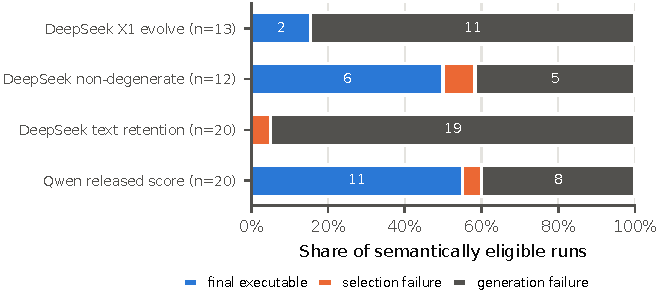
\includegraphics[width=\columnwidth]{figures/failure-decomposition.pdf}
\end{center}
\noindent\textit{Failure decomposition.} In every cohort most failed runs contain no parser-accepted executable candidate in the recorded pool (generation failures); selection failures, where a better selector over the same pool would have succeeded, total three of 46 failures.

\noindent\textit{Estimands and sensitivity.} The round-candidate-only oracle and the final-inclusive oracle are both 22/65, so the amendment below changes no value. Conditional on failure, generation failures are 43/46 (exact 95\% interval [0.821, 0.986]) and selection failures 3/46 ([0.014, 0.179]); as a share of eligible runs, recoverable failures are 3/65 ([0.010, 0.129]). Under reference exactness over all 72 runs, including the seven \texttt{\detokenize{IMPOSSIBLE}} references, the final and pool oracles are 19/72 and 22/72, the same three recoverable runs. Parser acceptance is 43/320 slots for DeepSeek X1 evolve, 95/192 for the non-degenerate arm, 52/320 for text retention, and 175/320 for Qwen (365/1,152 overall). Artifact 231 regenerates these numbers from the cached per-run rows.

\noindent\textit{Parser sensitivity.} The 43 generation failures average 13.6 rejected slots. Were each independently a false negative with probability 1\% (5\%), about 5.4 (21.0) of these runs would hold a valid candidate, so bounding a per-slot rate cannot certify the run count; that requires auditing every unique rejected text in the 46 failed runs (at most 495), which we have not done (artifact 237).


Protocol 080 freezes a zero-call extension to the 60-run DeepSeek X1 cohort, the 48-run non-degenerate main matrix, and the 40-run execution-aware confirmatory cohort. Semantic headroom excludes \texttt{\detokenize{IMPOSSIBLE}} references because forward execution cannot certify non-existence. Diversity and reference-exact summaries retain all runs. The original frozen estimand compared the 15-round-candidate oracle directly with the synthesized final. This comparison is not an upper bound because a synthesizer can in principle create a valid final absent from its input candidates. We retain the original protocol hash and record an outcome-aware amendment that adds the realized final to oracle support. The corrected quantity is weakly nonnegative and bounds selectors that can retain the current final. In the 65 selected semantically eligible original/control runs, the observed frequency of a valid synthesized final with no valid round-agent candidate is 0/65. No model call or run outcome changes.

Across original/control arms, empirical fixed-pool selector headroom is 0/13 for DeepSeek X1 evolve, 1/12 for DeepSeek non-degenerate original evolve, 1/20 for confirmatory text retention, and 1/20 for Qwen original scoring. An outcome-aware exploratory stratified synthesis gives 3/65=0.046, bootstrap interval [0, 0.108]. A two-sided Clopper--Pearson interval is [0.010, 0.129] if the heterogeneous cohorts are treated as exchangeable Bernoulli trials. This is an exact realized-pool bound for selectors restricted to the final plus 15 persisted round-agent candidates; population intervals concern similar-task generalization. Offline headroom in the confirmatory text-retention arm and the prospective execution-aware-minus-control point estimate are both 0.05 on the same 20 tasks, a descriptive convergence rather than an independent mediation test.

Exact-text repetition is provider-specific. Qwen original/length-zero duplicate rates are 0.809/0.822, whereas DeepSeek arms range approximately 0.073--0.272. Canonical parseable-plan support is consistently small: among 72 original/control runs, 38 have zero unique parseable canonical plans, 22 have one, 8 have two, and 4 have at least three. The arms average 0.45--1.05 unique canonical plans per run, and 73\%--91\% of parseable slots duplicate another canonical plan. We therefore distinguish lexical diversity from task-relevant candidate support.

\section{Stratified length synthesis and completeness diagnostic}

The 10-, 12-, and 20-pair length interventions contain 42 pairs. The stratified average exact difference is +0.0238, bootstrap interval [-0.0952, 0.1429], with four length-zero-only and three original-only successes and two-sided exact \(p=1\). This outcome-aware secondary synthesis meets the frozen rule for describing a precise near-zero average: its interval contains zero and its upper endpoint is below 0.15.

The length component's association with well-formed output does not transfer uniformly. DeepSeek original arms yield well-formed-prediction AUCs 0.938 and 1.0, but Qwen yields 0.133 with the opposite mean direction. Paired malformed changes under length removal are 0, -0.167, and +0.15. Thus length may act as a model-dependent formation proxy, but it is not a validated cross-model completeness or semantic-quality signal.

\section{Prospective candidate-pool enlargement}
\label{app:pool}

Protocol 083 was frozen before inspecting any output on 28 untouched reference-length-two PlanCraft tasks. Each task receives one complete uncached temperature-0 trajectory and five independent complete uncached temperature-0.7 trajectories. Thinking is disabled throughout. A trajectory contributes 15 round-agent answers and one synthesized final; canonical plans are deduplicated before support and execution measurement. The nested pool \(C_j\) contains the temperature-0 trajectory and stochastic repetitions 1 through \(j\). This makes \(C_5-C_1\) a randomized generation-budget contrast over an identical task set.

The eight-task gate passes: mean \(S_5-S_1=0.875\), 6/8 tasks have \(S_5\ge2\), all 48 valid trajectories complete five rounds, and all have positive usage. A provider payment interruption had previously created nine persisted traces containing \texttt{Access denied} or \texttt{overdue-payment}; an integrity back-audit marks all nine invalid, including two with partial positive usage. After seven valid tasks, the conservative 6.5M gate-token projection blocked the eighth task because those invalid attempts had consumed budget. The recorded amendment raises only this cap to 7.5M. The original and amended hashes begin \texttt{7ccf128c5bd4} and \texttt{97c35906de54}; the closure manifest stores both complete values. At amendment time, nested nonnegative support gains and the first seven task summaries made both substantive gate conditions mathematically irreversible. No task, condition, endpoint, threshold, or main budget changed.

The 20-task main cohort completes all 120 trajectories without an integrity failure. Results are:

\begin{center}
\resizebox{\columnwidth}{!}{%
\begin{tabular}{lrrrr}
\toprule
\textbf{Contrast} & \textbf{Mean difference} & \textbf{Task-bootstrap 95\% interval} & \textbf{One-sided 95\% lower bound} & \textbf{Exact test} \\
\midrule
Canonical support, \(C_5-C_1\) & +1.00 & [0.50, 1.60] & 0.60 & withdrawn: nested \\
Executable oracle, \(C_5-C_1\) & +0.20 & [0.05, 0.40] & 0.05 & withdrawn: nested \\
Headroom over baseline final, \(C_5-C_1\) & +0.20 & [0.05, 0.40] & 0.05 & withdrawn: nested \\
Standalone support, temperature 0.7 minus 0 & -0.05 & [-0.35, 0.25] & not applicable & \(p=1.0\) \\
\bottomrule
\end{tabular}%
}
\end{center}

The nested support/oracle/headroom curves are 1.85/0.60/0.10, 2.15/0.70/0.20, 2.35/0.70/0.20, 2.60/0.80/0.30, and 2.85/0.80/0.30 for \(C_1\) through \(C_5\). The originally reported nested sign-test values are invalid because decreases are excluded by construction and are formally withdrawn in artifact 088. The non-nested standalone temperature contrast permits either direction and retains its \(p=1\) result.

The trajectory decomposition contains 57 successful stochastic trajectories among 100. The anchor-inclusive plug-in oracle estimates are 0.660, 0.700, 0.722, 0.738, 0.751, 0.784, and 0.798 for \(n=1,2,3,4,5,10,\) and \(20\). The \(n>5\) values assume conditionally i.i.d. trajectories and are extrapolations. Task-cluster intervals, rather than trajectory-level independent intervals, preserve the 20-task experimental unit.

Per task, the nested oracle pattern from \(C_1\) to \(C_5\) is all-success for 12 tasks, all-failure for four, rescued at \(C_2\) for two, and rescued at \(C_4\) for two. Support gains \(C_5-C_1\) are 0 for eight tasks, 1 for eight, 2 for two, 3 for one, and 5 for one. Task-bootstrap intervals for the realized oracle are [0.40, 0.80] at \(C_1\), [0.50, 0.90] at \(C_2\) and \(C_3\), and [0.60, 0.95] at \(C_4\) and \(C_5\). Of the four \(C_5\)-only rescues, TEST0102, TEST0105, and TEST0361 contain a valid plan in 1/5 stochastic trajectories; TEST0526 contains one in 4/5. Five stochastic final answers alone attain 0.65 oracle coverage. A uniformly random final answer of \(C_j\) is executable 0.50, 0.52, 0.53, 0.55, and 0.54 of the time; the oracle's lead grows from 0.10 [0, 0.23] to 0.26 [0.10, 0.43]. A random stochastic slot is executable about 0.41 of the time. Score-based selectors cannot be replayed from the cached per-trajectory counts. At a matched count of 16 slots, cached cross-trajectory mixing has expected oracle 0.626 versus 0.570 within one stochastic trajectory, difference 0.056, task-bootstrap interval [0.016, 0.105]. All trajectories use the same three-agent runtime, so this is not a single-agent comparison.

Main-cohort generation costs are 4,807,489 recorded tokens for \(C_1\) and 14,430,644 for \(C_5\). The incremental four trajectories consume 9,623,155 tokens, a total ratio of 3.0017. Across gate and main, 168 valid trajectories record 10,546 calls and 20,489,906 tokens. Including the nine retained integrity-failed attempts gives 10,590 calls and 20,573,345 recorded tokens.

For cached \(C_5\) candidates, binary valid-versus-invalid executor utility gives \(g_U^{\mathrm{sel}}=\Delta_u=1\) and hence local \(\rho_U^{\mathrm{sel}}=1\) whenever a mixed-validity pool exists. This candidate-level ratio is distinct from the arm-level ablation consequence \(\delta_V^{\mathrm{abl}}\). The earlier artifact 071 conflated these estimands and its epsilon inversion is withdrawn; artifact 100 records the zero-call correction. The monotone exponential mechanism gives mean exact valid-selection probabilities 0.5119, 0.5748, 0.6822, 0.7793, and 0.7996 at \(\varepsilon=0.5, 1, 2, 4,\) and \(8\). These values are the expected consequence of a maximally separated binary signal on a small pool, not an independently discovered frontier. Under candidate-score replacement adjacency, one candidate's clipped validity bit may change and only the selected index/output is released; candidate text and the remaining system are trusted.

\section{Stopped DeepSeek compute-matched generation gate}
\label{app:repair}

Protocol 090 freezes a non-nested restart-versus-repair comparison before any provider call on 20 untouched reference-length-two tasks: eight adaptive gate candidates and 12 reserved main tasks. Each task receives a shared temperature-0 five-round, three-agent trajectory. An executable anchor-pool candidate causes symmetric success and zero added intervention calls. On anchor failure, a new temperature-0.7 trajectory defines realized token cap \(B_i\); sequential direct repair candidates count toward the primary pool only while cumulative repair tokens do not exceed \(B_i\). Repair uses the public task and reference-free executor diagnostic, never the hidden reference. Unsuccessful repair stops at its first budget crossing or 80 calls.

All eight gate tasks complete with provider integrity. Five anchors succeed, so only TEST0181, TEST0030, and TEST0535 are informative. Their outcomes are:

\begin{center}
\resizebox{\columnwidth}{!}{%
\begin{tabular}{lrrrrr}
\toprule
\textbf{Task} & \textbf{Restart} & \textbf{Repair} & \textbf{Restart tokens} & \textbf{Included repair tokens} & \textbf{Repair calls} \\
\midrule
TEST0181 & 0 & 1 & 157,910 & 1,008 & 1 \\
TEST0030 & 0 & 0 & 138,559 & 51,330 & 80 \\
TEST0535 & 0 & 0 & 162,193 & 50,313 & 80 \\
\bottomrule
\end{tabular}%
}
\end{center}

The frozen gate requires at least four informative anchor failures. It therefore stops even though repair has at least one rescue, does not underperform restart in rescue count, all provider records pass integrity, and both failed repair branches reach the 80-call exhaustion rule. No main task is run. Conditional on anchor failure, repair minus restart is +0.333 with task-bootstrap interval [0, 1] and exact paired \(p=1\). We do not interpret an all-eight difference because five symmetric successes are inherited from the shared anchor rather than caused by either intervention.

Repair diversity is the principal diagnostic. TEST0181 succeeds immediately with \texttt{\detokenize{["dark_oak_planks", "pink_bed"]}}; because it stops after one call, its modal concentration is not estimable. TEST0030 has only three raw response forms over 80 calls: 69 \texttt{\detokenize{["IMPOSSIBLE"]}}, nine \texttt{\detokenize{IMPOSSIBLE}}, and two empty responses. Its raw modal rate is 86.25\%, semantic normalization combines the first two forms into an \texttt{\detokenize{IMPOSSIBLE}} intent in 78/80 calls (97.5\%), and semantic pairwise agreement is 95.1\%. TEST0535 also has three raw forms, with \texttt{\detokenize{["redstone_torch"]}} appearing 76/80 times (95\% raw and semantic modal rates; 90.4\% semantic pairwise agreement); the missing intermediate \texttt{\detokenize{redstone}} makes it non-executable. Across the two exhausted tasks, the call-weighted raw modal share is 145/160=90.625\%, and the semantic share is 154/160=96.25\%.

The repair-only 0.80 threshold was introduced after observing the stopped gate and was not part of a frozen protocol. Calls within a task are not independent task units: the observed 86.25\%--95\% raw range comes from two failures only. Failure-type association is not estimable with three repair branches, and cross-cohort modal stability is unavailable because earlier disjoint DeepSeek cohorts did not record repeated direct repairs under this prompt. The executor behaves as intended in both failures: it does not certify \texttt{\detokenize{IMPOSSIBLE}}, and it rejects plans that omit required intermediate products.

We then froze protocol 096 before making a same-task public-only control. Each exhausted task received 80 additional DeepSeek temperature-0.7 calls with the same output-format instruction but no candidate, executor diagnostic, attempt index, response history, or reference. TEST0030 produced raw \texttt{\detokenize{["bookshelf"]}} in 79/80 calls (98.75\%), a different invalid mode from its repair-conditioned \texttt{\detokenize{["IMPOSSIBLE"]}}; TEST0535 produced raw \texttt{\detokenize{["redstone_torch"]}} in 76/80 and the same semantic plan in 80/80. No response was executable. Both tasks exceed the 0.80 near-determinism threshold frozen in protocol 096, and the mean task-level conditioned-minus-public-only raw modal-rate contrast is -0.0625. The control removes the candidate, diagnostic, attempt index, and history together, so it is not a single-factor intervention; it does not support conditioning as the cause. We use \textbf{task-level response collapse} for the repeated invalid endpoint under both direct prompts. Protocol 096 treats the two tasks as the independent units and forbids a call-level population test.

The first two direct calls on TEST0030 reached the output limit in hidden reasoning and exposed empty visible answers because the direct path omitted the full runtime's explicit non-thinking switch. Both calls, 3,768 tokens, and malformed outcomes remain in the intention-to-repair record; excluding them, TEST0030's raw modal rate is 69/78 (88.5\%) and its semantic modal rate 78/78. Subsequent direct calls pass \texttt{\detokenize{thinking.type=disabled}}; no prior output is deleted or rerun. LiteLLM response caching is disabled throughout, while DeepSeek's automatic provider-side prefix-cache accounting is separately outside that client flag. Total gate usage is 736 calls and 1,642,567 recorded tokens: 1,081,254 anchor, 458,662 restart, and 102,651 repair tokens. TEST0181 shows only that repair succeeded on its first attempt while a matched-budget restart failed; comparing first-draw tokens with a fully spent failed trajectory as a multiplicative efficiency ratio would be misleading. This stopped gate is positive mechanism evidence about two observed failures, but not a positive comparative-method claim.

\section{Held-out planning component control}
\label{app:planner}

The planner was developed post hoc on nine earlier PlanCraft screening tasks: DeepSeek selects one verifier-applicable recipe output per step, options are restricted to those with minimum finite post-action distance to the target, and a bounded symbolic pre-check (depth 12, 50,000 states) emits \texttt{IMPOSSIBLE} only when it exhausts its state space without a target. Its first held-out batch of nine tasks used an eight-step cap and truncated the three long tasks; the cap was then raised to 12 and the same batch rerun, after which a second batch of nine ran unchanged. Bounded stops are not global impossibility proofs. Reported separately: on the nine development tasks the final planner reached 7/7 feasible targets; the first held-out batch reached 3/6 feasible targets at the eight-step cap and 6/6 after the cap change; the untouched second batch reached 6/6 feasible targets with 4/6 canonical exact and 3/3 bounded stops. Only the second batch is a clean held-out evaluation. The final planning diagnostic used this frozen 18-task cohort and no new benchmark selection. The symbolic-only control reproduces 12/12 feasible replays, 8/12 canonical exact plans, six bounded stops on impossible-reference tasks, and 14/18 evaluator-exact labels. Ten of the 12 feasible cached plans are sequence-identical to the symbolic plans; the two remaining replay-valid plans use alternative action orderings. Only 7/78 accepted requests exposed multiple options, and four step-index mismatches occurred in two replay-valid tasks. These branch-level quantities are descriptive for the fixed cohort.

The prospective unfiltered DeepSeek arm removes bounded pre-checks and distance filtering but retains local action verification. It uses 142 provider calls and 43,623 recorded tokens, reaching 8/12 feasible targets with 5/12 canonical exact plans. Against symbolic search, replay has four symbolic-only and no live-only pairs (two-sided exact $p=0.125$); canonical matching has four symbolic-only and one live-only pair ($p=0.375$). The six impossible-reference runs terminate without reaching a target, which does not certify impossibility. This component comparison is separate from architecture-level inference and is not a causal multi-agent result.

\section{Closest work}
\label{app:closest}

\begin{center}
\resizebox{\columnwidth}{!}{%
\scriptsize
\begin{tabular}{lccccc}
\toprule
\textbf{Work} & \textbf{Adaptive extraction} & \textbf{Persistent state} & \textbf{Support bound} & \textbf{Private selector} & \textbf{Benchmark} \\
\midrule
MEXTRA \citep{wang2025mextra} & Yes & Agent memory & No & No & Memory-based agents \\
Agent TTS \citep{zhu2025ttsagents} & No & No & Partial & No & Agent benchmarks \\
This paper & No & Fixed-runtime state & Yes & Calculation only & PlanCraft \\
\bottomrule
\end{tabular}%
}
\end{center}

\section{Fixed-pool selector calculation}
\label{app:selector}

\noindent\textit{Setting.} The candidate set of a pool, its size $k$, and the output domain (the $k$ indices) are fixed and public. Each candidate $j$ has a clipped score $u_j\in[0,\Delta_u]$; here $u_j$ is binary executor validity and $\Delta_u=1$. Two inputs are neighbors under candidate-score replacement adjacency if they differ in the score of one candidate $i$ by at most $\Delta_u$. Candidate texts and everything else are trusted and unreleased.

\noindent\textit{Claim.} The mechanism $M$ that outputs $j$ with probability $w_j/Z$, where $w_j=\exp(\varepsilon u_j/\Delta_u)$ and $Z=\sum_l w_l$, is $\varepsilon$-DP under this adjacency.

\noindent\textit{Proof.} Let a neighbor raise $u_i$ by $\delta\in[0,\Delta_u]$, giving weights $w'$ and normalizer $Z'=Z+w_i(e^{\varepsilon\delta/\Delta_u}-1)$, so $Z\le Z'\le e^{\varepsilon\delta/\Delta_u}Z$. For $j=i$: $\Pr[M'=i]/\Pr[M=i]=e^{\varepsilon\delta/\Delta_u}Z/Z'\le e^{\varepsilon}$, and the reverse ratio is $e^{-\varepsilon\delta/\Delta_u}Z'/Z\le1$. For $j\ne i$: $\Pr[M'=j]/\Pr[M=j]=Z/Z'\le1$ and the reverse ratio is $Z'/Z\le e^{\varepsilon}$. A decrease is symmetric. This is the monotone case of the exponential mechanism \citep{mcsherry2007mechanism}; under adjacencies where several scores can move in opposite directions, the general calibration $\exp(\varepsilon u_j/2\Delta_u)$ is required, which doubles every budget.

\begin{center}
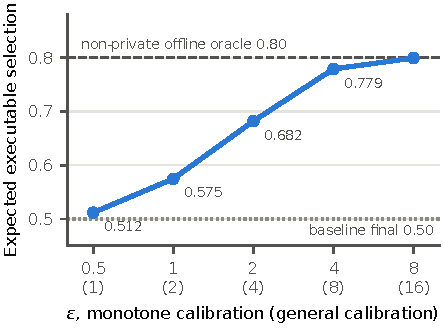
\includegraphics[width=0.85\columnwidth]{figures/selector-calculation.pdf}
\end{center}
\noindent\textit{Values.} Means over the 20 cached $C_5$ pools (pools without a valid candidate contribute 0, so the ceiling is the 0.80 offline oracle). Labels give $\varepsilon$ under the monotone calibration with the general-calibration equivalent in parentheses. This is not a deployed selector, not a privacy--utility frontier, and not end-to-end privacy.

\section{Reproducibility supplement}
\label{app:repro}

The anonymous supplement contains the frozen protocols released with this paper, the cached analyses 037, 080, 081, 087, and 088, the replication summary 223, and our analysis, reanalysis, and figure scripts. Running the reanalysis script regenerates the counts in Table~\ref{tab:headroom}, the generation- and selection-failure counts and intervals, the parser acceptance rates, the per-task pool patterns and intervals of Figure~\ref{fig:pool}, the score-source counts of Figure~\ref{fig:audit}c, and the canary denominators; artifact 237 adds the random-final baselines, endpoint comparison, and parser sensitivity; the figure script redraws Figures~\ref{fig:audit} and~\ref{fig:pool} and the appendix figures. The upstream TacoMAS runtime is not redistributed because its license could not be confirmed, so live runs require a separate checkout. Models are DeepSeek V4 Flash and the dated \texttt{\detokenize{qwen3.7-max-2026-06-08}} snapshot, with thinking disabled, client-side response caching disabled, temperature 0 for anchors and audits, and temperature 0.7 for stochastic trajectories, repairs, and public-only calls. The PlanCraft task file used by the replication has SHA-256 prefix \texttt{1d41af11279c}.

